\documentclass[12pt]{article}

\usepackage{fancyhdr}
\usepackage{amssymb}
\usepackage{amsthm}
\usepackage{amsfonts}
\usepackage{mathtools}
\usepackage{array}
\usepackage{systeme}
\usepackage{geometry}
\usepackage{enumitem}
\usepackage{ dsfont }
\usepackage{listings}
\usepackage{booktabs}
\usepackage{hyperref}
\usepackage{tikz}
\usetikzlibrary{arrows,decorations.pathmorphing,backgrounds,positioning,fit}
\usetikzlibrary{automata, positioning}
\usetikzlibrary{calc}
\usepackage[utf8]{inputenc}
  \geometry{
    left = 2.5cm,
    right = 2.5cm,
    includeheadfoot, top = 1.5cm, bottom = 1.5cm,
    headsep = 1.3cm,
    footskip = 1.2cm
  }

% Inline fraction %
\newcommand*\rfrac[2]{{}^{#1}\!/_{#2}}
\newcommand{\lincom}[4]{\mathit{{#1}{\underline{#2}}}+\mathit{{#3}{\underline{#4}}}}
\newcommand*{\QEDA}{\hfill\ensuremath{\blacksquare}}
\newcommand*{\QEDB}{\hfill\ensuremath{\square}}
\newcommand{\MU}[1]{\mathit{\underline{#1}}}

\newcommand{\DS}{\displaystyle}
\newcommand{\bb}[1]{\mathbb{#1}}

% Absolute value: \abs{x} => |x|
\newcommand{\abs}[1]{\left|#1\right|}

% Function: \func{f}{X}{Y} => f : X -> Y
\newcommand{\func}[3]{#1 : #2 \rightarrow #3}
% Function to R: \func{f}{X} => f : X -> R
\newcommand{\functoR}[2]{#1 : #2 \rightarrow \mathbb{R}}
% Function to N: \func{f}{X} => f : X -> N
\newcommand{\functoN}[2]{#1 : #2 \rightarrow \mathbb{N}}
% Function from R to R: \func{f} => f : R -> R
\newcommand{\funcR}[1]{#1 : \mathbb{R} \rightarrow \mathbb{R}}

% Limits and convergence
\newcommand{\limn}{\lim_{n \to \infty}}
\newcommand{\limh}{\lim_{h \to 0}}
\newcommand{\limsupn}{\limsup_{n \to \infty}}
\newcommand{\liminfn}{\liminf_{n \to \infty}}
\newcommand{\limx}[1]{\lim_{x \to #1}}
\newcommand{\tounif}{\xrightarrow{unif.}}

% Sums and series
\newcommand{\sumn}[1]{\sum_{k=1}^n #1}
\newcommand{\series}[1]{\sum_{k=1}^\infty #1}
\newcommand{\seriec}[1]{\sum_{k=m}^n #1}
\newcommand{\pseries}[1]{\sum_{n=0}^\infty #1}

% Intervals
% Closed-closed interval [a,b]
\newcommand{\intcc}[1]{\left[#1\right]}
% Open-closed interval (a,b]
\newcommand{\intoc}[1]{\left(#1\right]}
% Closed-open interval [a,b)
\newcommand{\intco}[1]{\left[#1\right)}
% Open-open interval (a,b)
\newcommand{\intoo}[1]{\left(#1\right)}

% Sets
\newcommand{\N}{\mathbb{N}}
\newcommand{\Z}{\mathbb{Z}}
\newcommand{\Q}{\mathbb{Q}}
\newcommand{\R}{\mathbb{R}}
\newcommand{\e}{\varepsilon}

\lhead{Alexander Fischer, Camillo Malnati, Federico Pfahler, Aldo Gabriele di Rosa}
\chead{}
\rhead{}
\rfoot{\thepage}
\cfoot{}
\lfoot{\today}
\pagestyle{fancy}

\begin{document}
  \begin{center}
    \LARGE{\textbf{MindPollution}}
  \end{center}
  \section{Introduction}
  \newpage
  \section{Architecture}

  Figure~\ref{fig:architecture} shows an overview of the architecture of our project, showing the main components.
  \begin{figure}[ht]
    \centering
    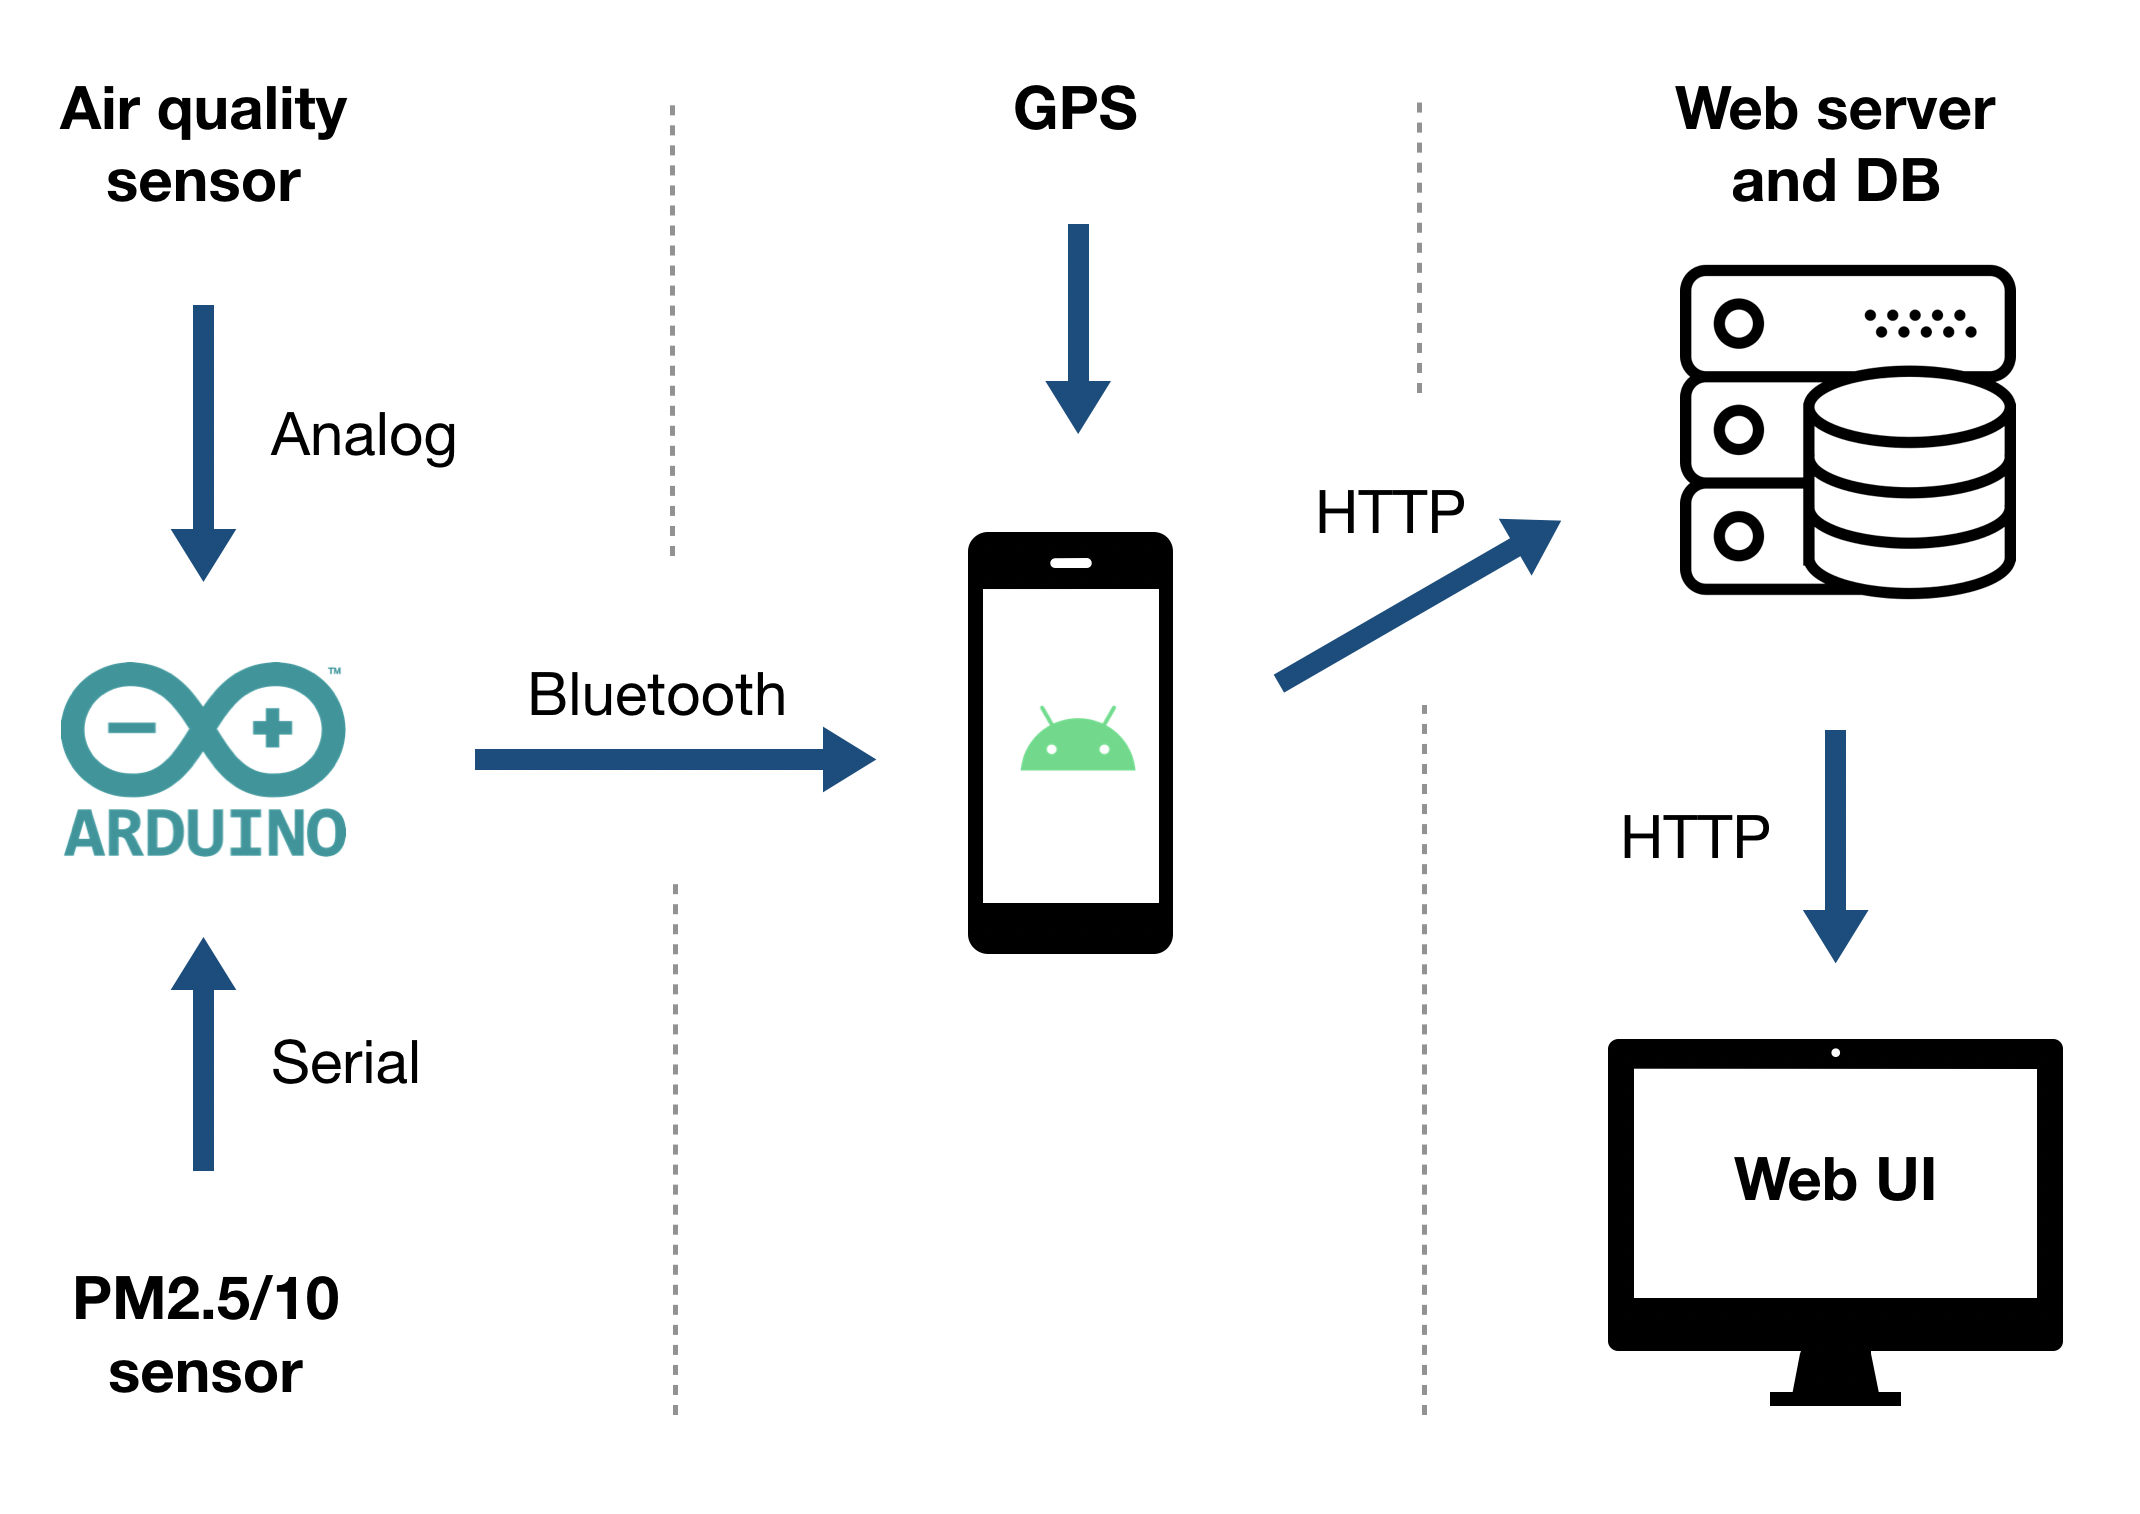
\includegraphics[width=\textwidth]{images/architecture.png}
    \caption{An overview of the main components in our system.}
    \label{fig:architecture}
  \end{figure}
  \subsection{Sensors}
  To measure the air quality and pollutions levels we use two sensors that we connect directly to the Arduino board.
  \subsubsection{Air quality}
  We measure the air quality by using a module that includes a MQ-135 gas sensor (see datasheet\footnote{https://www.olimex.com/Products/Components/Sensors/Gas/SNS-MQ135/resources/SNS-MQ135.pdf}), which is sensitive to several pollutants including $NH_3$, $NO_x$, alcohol, benzene, smoke and $CO_2$.
  Its output is an aggregated level of \textit{air quality}, either as an analog voltage or as a digital output based on a threshold. An higher value implies that the density of the detected gases is higher, and therefore the air quality is worse.

  This module requires a supply voltage of $5\ volts$, and we connect its analog output to an analog input pin (i.e. $A0$) of our Arduino Nano board.
  %TODO: add photo

  \subsubsection{Particulate matter (PM2.5/PM10)}
  Another sensor that we use to measure the pollution is the Nova Fitness SDS011 (see datasheet\footnote{https://cdn-reichelt.de/documents/datenblatt/X200/SDS011-DATASHEET.pdf}), which measures the density of particulate matter (i.e. PM2.5 and PM10) in the air. Its range of measured values is between $0$ and $999\mu/gm^3$.

  To output those values, the module has a serial interface based on the UART communication protocol, described in \autoref{fig:uart-protocol}, and the rate of transmission of the measurements is $1Hz$. We connected the output pin of this serial interface to the serial input pin of our Arduino Nano board. Furthermore, similarly to the air quality sensor, the module requires a supply voltage of $5\ volts$.

  %TODO: add photo

  \begin{figure}[ht]
    \centering
    \begin{tabular}{r | l | l}
      \# & Name & Content\\\toprule
      0 & Header & AA\\
      1 & Commander No. & C0\\
      2 & DATA 1 & PM2.5 Low Byte\\
      3 & DATA 2 & PM2.5 High Byte\\
      4 & DATA 3 & PM10 Low Byte\\
      5 & DATA 4 & PM10 High Byte\\
      6 & DATA 5 & ID Byte 1\\
      7 & DATA 6 & ID Byte 2\\
      8 & Checksum & Checksum\\
      9 & Tail & AB\\
    \end{tabular}
    \caption{The bytes sent over the serial interface}
    \label{fig:uart-protocol}
  \end{figure}
  \subsection{Android application}
  The goal of the Android application is to act as a \textit{gateway} between the Arduino board that collects pollution data from sensors and the web application that stores and visualizes the aggregated data. While forwarding pollution measurements, it also adds the current location coordinates obtained from the phone's GPS sensor.

  The application runs on a mobile phone (in our demo a Huawei P10 lite running Android 8.0) that is connected via Bluetooth to the Arduino Nano 33 BLE board, as well as with an active GSM connection.
  Its source code is based on an example application, \verb|BluetoothLeGatt|, which is bundled with the official Android SDK, that allows to scan for Bluetooth Low Energy devices and connect to them. 

  What we added to that code was to, on every message received from the Arduino board, retrieve the location coordinates (using the Android FusedLocation API) and send that data together with the pollution information to a web server as a JSON object by performing a POST request. An example of such JSON object is shown in Figure~\ref{lst:json-packet}. On the other hand, the message sent from the board is structured as follows: \verb|123,12,5;|. It contains the measurements from the air quality sensor, as well as the two measured values from the PM2.5/10 sensor.

  %TODO: add screenshots of app

  \begin{figure}[h]
    \centering
    \begin{verbatim}
{
  "createdAt": "2019-12-13T09:22:49.824Z",
  "lat": 46.0037,
  "long": 8.9511 ,
  "bikeId" : "00002add-0000-1000-8000-00805f9b34fb",
  "pm10": 5,
  "pm25": 12,
  "airQuality": 123
}
    \end{verbatim}
  \caption{An example JSON object containing the pollution measurements and location}\label{lst:json-packet}
  \end{figure}

  \subsection{Web application}
  \newpage
  \section{Conclusions}
  

\end{document}
